% Options for packages loaded elsewhere
\PassOptionsToPackage{unicode}{hyperref}
\PassOptionsToPackage{hyphens}{url}
%
\documentclass[
]{article}
\usepackage{amsmath,amssymb}
\usepackage{lmodern}
\usepackage{wrapfig}
\usepackage{iftex}
\ifPDFTeX
  \usepackage[T1]{fontenc}
  \usepackage[utf8]{inputenc}
  \usepackage{textcomp} % provide euro and other symbols
\else % if luatex or xetex
  \usepackage{unicode-math}
  \defaultfontfeatures{Scale=MatchLowercase}
  \defaultfontfeatures[\rmfamily]{Ligatures=TeX,Scale=1}
\fi
% Use upquote if available, for straight quotes in verbatim environments
\IfFileExists{upquote.sty}{\usepackage{upquote}}{}
\IfFileExists{microtype.sty}{% use microtype if available
  \usepackage[]{microtype}
  \UseMicrotypeSet[protrusion]{basicmath} % disable protrusion for tt fonts
}{}
\makeatletter
\@ifundefined{KOMAClassName}{% if non-KOMA class
  \IfFileExists{parskip.sty}{%
    \usepackage{parskip}
  }{% else
    \setlength{\parindent}{0pt}
    \setlength{\parskip}{6pt plus 2pt minus 1pt}}
}{% if KOMA class
  \KOMAoptions{parskip=half}}
\makeatother
\usepackage{xcolor}
\usepackage[margin=1in]{geometry}
\usepackage{color}
\usepackage{fancyvrb}
\newcommand{\VerbBar}{|}
\newcommand{\VERB}{\Verb[commandchars=\\\{\}]}
\DefineVerbatimEnvironment{Highlighting}{Verbatim}{commandchars=\\\{\}}
% Add ',fontsize=\small' for more characters per line
\usepackage{framed}
\definecolor{shadecolor}{RGB}{248,248,248}
\newenvironment{Shaded}{\begin{snugshade}}{\end{snugshade}}
\newcommand{\AlertTok}[1]{\textcolor[rgb]{0.94,0.16,0.16}{#1}}
\newcommand{\AnnotationTok}[1]{\textcolor[rgb]{0.56,0.35,0.01}{\textbf{\textit{#1}}}}
\newcommand{\AttributeTok}[1]{\textcolor[rgb]{0.77,0.63,0.00}{#1}}
\newcommand{\BaseNTok}[1]{\textcolor[rgb]{0.00,0.00,0.81}{#1}}
\newcommand{\BuiltInTok}[1]{#1}
\newcommand{\CharTok}[1]{\textcolor[rgb]{0.31,0.60,0.02}{#1}}
\newcommand{\CommentTok}[1]{\textcolor[rgb]{0.56,0.35,0.01}{\textit{#1}}}
\newcommand{\CommentVarTok}[1]{\textcolor[rgb]{0.56,0.35,0.01}{\textbf{\textit{#1}}}}
\newcommand{\ConstantTok}[1]{\textcolor[rgb]{0.00,0.00,0.00}{#1}}
\newcommand{\ControlFlowTok}[1]{\textcolor[rgb]{0.13,0.29,0.53}{\textbf{#1}}}
\newcommand{\DataTypeTok}[1]{\textcolor[rgb]{0.13,0.29,0.53}{#1}}
\newcommand{\DecValTok}[1]{\textcolor[rgb]{0.00,0.00,0.81}{#1}}
\newcommand{\DocumentationTok}[1]{\textcolor[rgb]{0.56,0.35,0.01}{\textbf{\textit{#1}}}}
\newcommand{\ErrorTok}[1]{\textcolor[rgb]{0.64,0.00,0.00}{\textbf{#1}}}
\newcommand{\ExtensionTok}[1]{#1}
\newcommand{\FloatTok}[1]{\textcolor[rgb]{0.00,0.00,0.81}{#1}}
\newcommand{\FunctionTok}[1]{\textcolor[rgb]{0.00,0.00,0.00}{#1}}
\newcommand{\ImportTok}[1]{#1}
\newcommand{\InformationTok}[1]{\textcolor[rgb]{0.56,0.35,0.01}{\textbf{\textit{#1}}}}
\newcommand{\KeywordTok}[1]{\textcolor[rgb]{0.13,0.29,0.53}{\textbf{#1}}}
\newcommand{\NormalTok}[1]{#1}
\newcommand{\OperatorTok}[1]{\textcolor[rgb]{0.81,0.36,0.00}{\textbf{#1}}}
\newcommand{\OtherTok}[1]{\textcolor[rgb]{0.56,0.35,0.01}{#1}}
\newcommand{\PreprocessorTok}[1]{\textcolor[rgb]{0.56,0.35,0.01}{\textit{#1}}}
\newcommand{\RegionMarkerTok}[1]{#1}
\newcommand{\SpecialCharTok}[1]{\textcolor[rgb]{0.00,0.00,0.00}{#1}}
\newcommand{\SpecialStringTok}[1]{\textcolor[rgb]{0.31,0.60,0.02}{#1}}
\newcommand{\StringTok}[1]{\textcolor[rgb]{0.31,0.60,0.02}{#1}}
\newcommand{\VariableTok}[1]{\textcolor[rgb]{0.00,0.00,0.00}{#1}}
\newcommand{\VerbatimStringTok}[1]{\textcolor[rgb]{0.31,0.60,0.02}{#1}}
\newcommand{\WarningTok}[1]{\textcolor[rgb]{0.56,0.35,0.01}{\textbf{\textit{#1}}}}
\usepackage{longtable,booktabs,array}
\usepackage{calc} % for calculating minipage widths
% Correct order of tables after \paragraph or \subparagraph
\usepackage{etoolbox}
\makeatletter
\patchcmd\longtable{\par}{\if@noskipsec\mbox{}\fi\par}{}{}
\makeatother
% Allow footnotes in longtable head/foot
\IfFileExists{footnotehyper.sty}{\usepackage{footnotehyper}}{\usepackage{footnote}}
\makesavenoteenv{longtable}
\usepackage{graphicx}
\makeatletter
\def\maxwidth{\ifdim\Gin@nat@width>\linewidth\linewidth\else\Gin@nat@width\fi}
\def\maxheight{\ifdim\Gin@nat@height>\textheight\textheight\else\Gin@nat@height\fi}
\makeatother
% Scale images if necessary, so that they will not overflow the page
% margins by default, and it is still possible to overwrite the defaults
% using explicit options in \includegraphics[width, height, ...]{}
\setkeys{Gin}{width=\maxwidth,height=\maxheight,keepaspectratio}
% Set default figure placement to htbp
\makeatletter
\def\fps@figure{htbp}
\makeatother
\setlength{\emergencystretch}{3em} % prevent overfull lines
\providecommand{\tightlist}{%
  \setlength{\itemsep}{0pt}\setlength{\parskip}{0pt}}
\setcounter{secnumdepth}{-\maxdimen} % remove section numbering
\newcommand{\beginsupplement}{\setcounter{table}{0} \renewcommand{\thetable}{S\arabic{table}} \setcounter{figure}{0} \renewcommand{\thefigure}{S\arabic{figure}}}
\ifLuaTeX
  \usepackage{selnolig}  % disable illegal ligatures
\fi
\IfFileExists{bookmark.sty}{\usepackage{bookmark}}{\usepackage{hyperref}}
\IfFileExists{xurl.sty}{\usepackage{xurl}}{} % add URL line breaks if available
\urlstyle{same} % disable monospaced font for URLs
\hypersetup{
  pdftitle={Supplementary Materials 2 - ARGweaver Analysis},
  pdfauthor={Daria Shipilina, Arka Pal, Sean Stankowski, Yingguang Frank Chan, Nicholas H. Barton},
  hidelinks,
  pdfcreator={LaTeX via pandoc}}

\title{Supplementary Materials 2 - ARGweaver Analysis}
\author{Daria Shipilina, Arka Pal, Sean Stankowski, Yingguang Frank Chan, Nicholas H. Barton}
\date{}

\begin{document}
\maketitle

\begin{center}\rule{0.5\linewidth}{0.5pt}\end{center}

\hfill\break
\setcounter{table}{0} \renewcommand{\thetable}{S\arabic{table}} \setcounter{figure}{0} \renewcommand{\thefigure}{S\arabic{figure}}

This document outlines the pipeline followed to obtain
\textbf{Figure 6}. The associated
\href{https://github.com/DaSh-bash/Suppl_Materials_On_the_origin_2022}{.Rmd
file} (https://github.com/DaSh-bash/Suppl\_Materials\_On\_the\_origin\_2022/Supplement-Information-2.Rmd) provides the detailed code to reproduce results.

\hypertarget{running-argweaver}{%
\subsection{1. Running ARGweaver}\label{running-argweaver}}

\hypertarget{sample-information}{%
\paragraph{\texorpdfstring{1.1. Sample information\\
}{1.1. Sample information }}\label{sample-information}}

\hfill\break
ARGweaver is applied on a phased SNP dataset of \emph{Heliconius
erato} butterflies, sequenced by \emph{haplotagging}, a technique that
produces linked-read sequence data. We used two previously
published genomic regions - \emph{Herato1801:1362067-1405605} (coincides
with the previously identified gene \emph{optix} that has undergone a
selective sweep) and \emph{Herato1603:3450000-3493538} (a neutral
background region) (Meier et al, 2021). 10 individuals of
\emph{H.e.lativitta} and \emph{H.e.notabilis} were chosen from opposite
ends of the hybrid zone transect for ARG inference.

\hypertarget{preprocessing-files-for-argweaver}{%
\paragraph{\texorpdfstring{1.2. Preprocessing files for ARGweaver\\
}{1.2. Preprocessing files for ARGweaver }}\label{preprocessing-files-for-argweaver}}

\hfill\break
To preprocess the input files for ARGweaver, we first subset the 20
diploid individuals from full VCF files (see Supplementary Information
in \href{https://www.pnas.org/doi/10.1073/pnas.2015005118}{Meier et al,
2021}), and then convert the SNP information into the \emph{.sites}
format required by ARGweaver. The \emph{.sites} format only contains
information on the positions that are varying within the 20 individuals
that we chose.

In the \textit{optix} region (43538 bp long), there are 2812 sites
altogether - 2426 are variant positions, while 330 and 56 sites are
fixed for one or the other allele. Genomic positions that are neither
variant nor fixed to one or the other allele (in other words, positions
absent in the VCF file) are considered missing information and therefore
masked from being used as input data for ARGweaver. Altogether,
ARGweaver uses information of variant alleles and invariant alleles;
whereas the rest is masked and treated as missing information.

Similiarly, the neutral region, \emph{Herato1603:3450000-3493538}
(43538 bp) has 6407 sites altogether - 4926 is variant positions, while
1405 and 76 sites are fixed for either allele.

\hypertarget{input-parameters}{%
\paragraph{\texorpdfstring{1.3. Input parameters\\
}{1.3. Input parameters }}\label{input-parameters}}

\hfill\break
In order to run ARGweaver, we consider mutation rate,
\(\mu = 2.9 \times 10^{-9}\) per bp per generation, and its ratio to
recombination rate, \(\frac{\mu}{r}\) = 1. We estimate \(N_e\) by
calculating Tajima's \(\pi\) (= \(4N_e r\)) from the neutral region.
\(\pi\) = 0.0225049, \(N_e\) = 1940078. The total map length of both
\emph{optix} and neutral region is 0.01262602 cM.\\

\begin{Shaded}
\begin{Highlighting}[]
\DocumentationTok{\#\# Calculating Ne from Herato1603:3450000{-}3550000}

\NormalTok{r }\OtherTok{=} \FloatTok{2.9e{-}09}  \CommentTok{\# recombination rate}
\NormalTok{L }\OtherTok{=} \DecValTok{3550000} \SpecialCharTok{{-}} \DecValTok{3450000}  \CommentTok{\# Genomic length}
\NormalTok{n }\OtherTok{=} \DecValTok{40}  \CommentTok{\# no. of samples}
\NormalTok{pi\_sum }\OtherTok{=} \FloatTok{2250.49}  \CommentTok{\# Sum of pi estimates across all sites}
\NormalTok{pi }\OtherTok{=}\NormalTok{ pi\_sum}\SpecialCharTok{/}\NormalTok{L  }\CommentTok{\# pi estimate}
\NormalTok{S }\OtherTok{=} \DecValTok{10571}  \CommentTok{\# No of seggregating sites in this region }
\NormalTok{Ne\_tajima }\OtherTok{=}\NormalTok{ pi}\SpecialCharTok{/}\NormalTok{(}\DecValTok{4} \SpecialCharTok{*}\NormalTok{ r)  }\CommentTok{\# Tajima\textquotesingle{}s Ne}
\NormalTok{Ne\_watterson }\OtherTok{=}\NormalTok{ S}\SpecialCharTok{/}\NormalTok{(}\DecValTok{4} \SpecialCharTok{*}\NormalTok{ r }\SpecialCharTok{*}\NormalTok{ L) }\SpecialCharTok{*}\NormalTok{ (}\FunctionTok{sum}\NormalTok{(}\FunctionTok{c}\NormalTok{(}\DecValTok{1}\SpecialCharTok{:}\NormalTok{(n }\SpecialCharTok{{-}} \DecValTok{1}\NormalTok{))}\SpecialCharTok{\^{}}\NormalTok{(}\SpecialCharTok{{-}}\DecValTok{1}\NormalTok{)))}\SpecialCharTok{\^{}{-}}\DecValTok{1}  \CommentTok{\# Waterson\textquotesingle{}s Ne}
\end{Highlighting}
\end{Shaded}

\begin{verbatim}
## pi = 0.0225049 
## Ne_tajima = 1940078 
## Ne_watterson = 2142433 
## Ne_tajima/Ne_watterson = 0.9055488
## Map Length = 0.01262602 cM
\end{verbatim}

ARGweaver allows coalescence and recombination events to take place only at discretized time points, defined by the function, \(t(i)=\frac {exp(\frac{ i}{K−1}log(1+\delta t_{max}))−1}{\delta}\); for \emph{K} time points and \(i\in{\{0, 1, …, K−1\}}\). Very small values of \(\delta ( <\frac {1}{t_{max}})\) will yield roughly linear
distribution of times, whereas larger values of \(\delta\) will place
more time points in recent past and less in deep past. For this
analysis, we set \emph{K} = 30, the maximum time for total coalescence
(\(t_{max}\)) = 20\(N_e\), and the shape parameter (\(\delta\)) = 0.01
(\emph{Figure S1}).

\begin{figure}
{\centering \includegraphics[width=0.50\textwidth]{figS1-Discrete-Time-points-1} }
\caption{ \footnotesize Discrete time points for ARGweaver analysis - 30 time steps, $N_e$ = 1940078, Left y-axis shows the time points in $N_e$, while right y-axis in number of generations. Red line denotes 1$N_e$.}\label{fig:figS1-Discrete-Time-points}
\end{figure}


\paragraph{\texorpdfstring{1.4. Run ARGweaver\\
}{1.4. Run ARGweaver }}\label{run-argweaver}}
\hfill\break
ARGweaver is run for 5000 iterations and then resumed for another 5000
iterations for the \emph{optix} region, whereas only 5000 iterations for
the neutral region.\\

\begin{Shaded}
\begin{Highlighting}[]
\CommentTok{\# Run ARGweaver}
\ExtensionTok{\textasciitilde{}/.local/bin/arg{-}sample} \AttributeTok{{-}s}\NormalTok{  sites/}\VariableTok{$\{regionName\}}\NormalTok{\_Herato.sites }\DataTypeTok{\textbackslash{}}
    \AttributeTok{{-}{-}maskmap}\NormalTok{ masks/}\VariableTok{$\{regionName\}}\NormalTok{\_Herato\_mask.bed.gz }\DataTypeTok{\textbackslash{}}
    \AttributeTok{{-}N}\NormalTok{ 1940078 }\AttributeTok{{-}m}\NormalTok{ 2.9e{-}9 }\AttributeTok{{-}r}\NormalTok{ 2.9e{-}9 }\AttributeTok{{-}{-}ntimes}\NormalTok{ 30 }\DataTypeTok{\textbackslash{}}
    \AttributeTok{{-}{-}maxtime} \VariableTok{$((}\DecValTok{1940078}\OperatorTok{*}\DecValTok{20}\VariableTok{))} \AttributeTok{{-}{-}iters}\NormalTok{ 10000 }\AttributeTok{{-}{-}delta}\NormalTok{ 0.01 }\DataTypeTok{\textbackslash{}}
    \AttributeTok{{-}{-}output}\NormalTok{ \{regionName\}/sample/}\VariableTok{$\{regionName\}}
\end{Highlighting}
\end{Shaded}


\hypertarget{analysis-of-argweaver-output}{%
\subsection{\texorpdfstring{2. Analysis of ARGweaver output\\
}{2. Analysis of ARGweaver output }}\label{analysis-of-argweaver-output}}

\hypertarget{mcmc-summary}{%
\paragraph{\texorpdfstring{2.1. MCMC summary\\
}{2.1. MCMC summary }}\label{mcmc-summary}}

\hfill\break
After visualizing MCMC traces of likelihood, prior and joint
probabilities, we decided to set the first 3000 iterations as burnin.
The plot below is for the \emph{optix} region (\emph{Figure S2}).

\begin{figure}
{\centering \includegraphics{figS2-MCMC-parameters-OPTIX-1} 

}

\caption{\footnotesize Traces across all MCMC iterations of prior (log probability of the sampled ARG given the model), likelihood (log probability of the data given the sampled ARG), joint - (total log probability of the ARG and the data; prior + likelihood), recombs - (number of recombination events in the sampled ARG), arglen (total length of all branches summed across sites) and noncompats (number of variant sites that cannot be explained by infinite sites mutation model)}.}\label{fig:figS2-MCMC-parameters-OPTIX}
\end{figure}

\hypertarget{argweaver-output}{%
\paragraph{\texorpdfstring{2.2. ARGweaver output\\
}{2.2. ARGweaver output }}\label{argweaver-output}}

\hfill\break
The ARGweaver output, \emph{.smc} files are then converted to
\emph{.bed} format to extract TMRCAs, trees, recomination breakpoints
and total tree branch lengths across all iterations (except burnin). Two
iterations (Iteration 8250 and 9200) are chosen for further analysis and
identification of haplotype blocks.

\hypertarget{tmrca}{%
\paragraph{\texorpdfstring{2.3. TMRCA\\
}{2.3. TMRCA }}\label{tmrca}}
\hfill\break
We first examine the TMRCA of the total tree and the individual
populations - \emph{H.e.lativitta} (in red) and \emph{H.e.notabilis} (in
yellow) (\emph{Figure S3}). Unlike the neutral region
(\emph{Herato1603}) where all TMRCA estimates are fairly constrained
between 1 and 10 \(N_e\), TMRCA traces for individual populations in the
\emph{optix} region exhibit shallow coalescence times at multiple
positions throughout the entire \textasciitilde50kb region. In case of a
selective sweeps, where a beneficial mutation sweeps through the
population, TMRCA tends to be shallow since all samples in the swept
population coalesces quickly to the initial ``lucky'' ancestor. Moving
away from the focal mutations, lineages recombine away from the swept
ancestral background. The TMRCA estimates from the \emph{optix} region
is consistent with the previously identified selected region in
\emph{optix}. To investigate further the haplotype block structures, we
focus into a 3kb region at optix:1385966-1388966.

\begin{figure}
{\centering \includegraphics{figS3-TMRCA-1} }
\caption{ \footnotesize TMRCA ($N_e$) for each position in the \textit{optix} and the \textit{neutral} genomic region. Black line: total TMRCA, Red: Median TMRCA for \textit{H.e.lativitta}, Yellow: TMRCA for \textit{H.e.notabilis}. Corresponding shaded regions are the 0.05 and 0.95 percentile intervals.}\label{fig:figS3-TMRCA}
\end{figure}

In the focal region, there are 137 SNPs. SNPs are changed from its
nucleotide assignment to 0/1; based on allele frequency within the
\emph{H.e.lativitta} samples. (Higher allele frequency - 1, Lower allele
frequency - 0)

\begin{figure}
{\centering 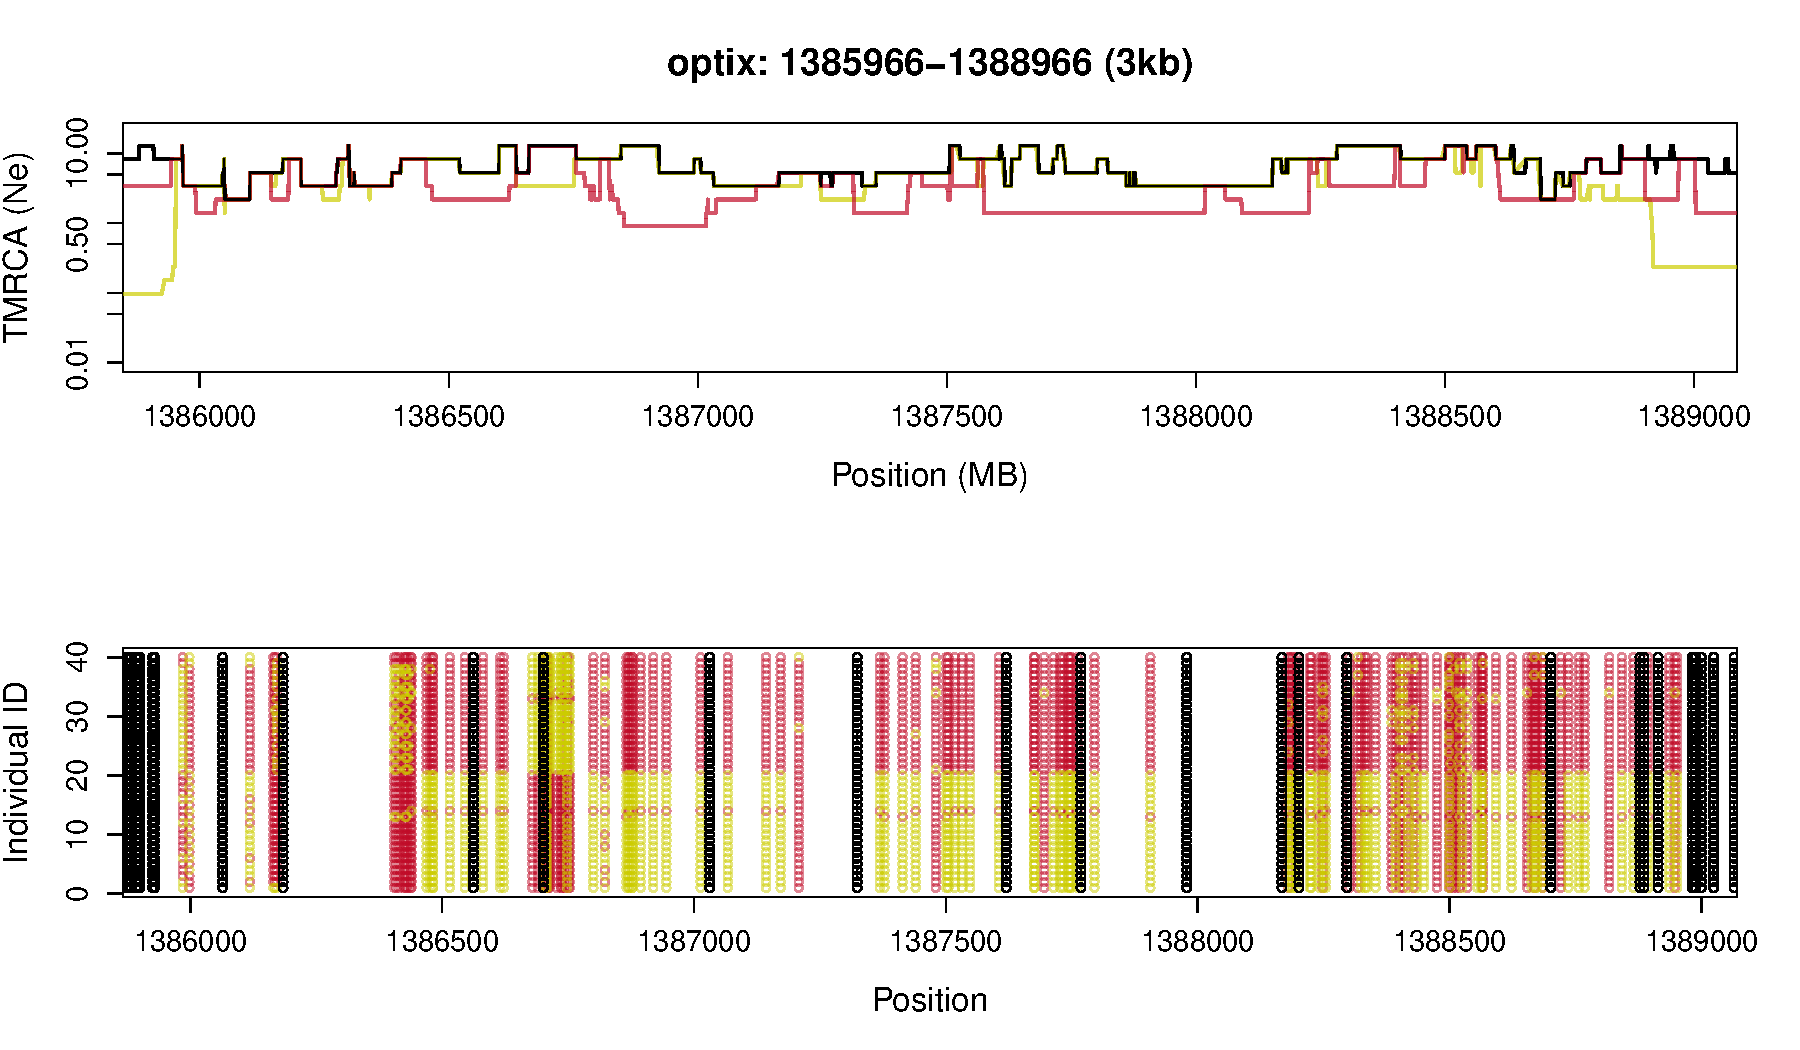
\includegraphics[width=0.99\textwidth]{figS4-focal-SNPs/TMRCA-1} 
}

\caption{ \footnotesize TMRCA for each position in focal genomic region (optix:1385966-1388966). Same colour schemes as above. \textbf{Top panel:} TMRCA plot, \textbf{Bottom panel:} SNPs in both populations; RED and YELLOW alleles are variant positions, coloured according to the respective higher and lower allele counts in the \textit{H.e.lativitta} population. BLACK alleles are fixed (invariant) in both populations. All other positions (in white) are unknown, since those positions do not have SNP information. These unknown positions are masked while running ARGWeaver, therefore they are treated as missing information and NOT as invariant sites.}\label{fig:figS4-focal-SNPs/TMRCA}
\end{figure}

Masking sites can have a critical effect on sampling ARGs, since
invariant sites can shift priors towards a recent coalescence (because
there hasn't been enough time yet for a mutation to occur in any of the
branches), whereas missing information does not shift priors and
therefore ARGs are sampled neutrally in those regions. In the above
region of 3kb, there are 137 SNPs and 16 invariant positions. Out of the
137 SNPs, only 59 SNPs are segregating within the \emph{H.e.lativitta}
population in focus (\emph{Figure S4})

Hereafter, alleles with lower frequency within the
\emph{H.e.lativitta} population is referred to as the minor allele, and
individuals who share the minor allele is the minor clade. Conversely,
individuals that carry that major allele is called major clade. Minor
allele is coded as 0 and major as 1.

\hypertarget{general-comments-on-identifying-haplotype-blocks-as-edges-from-empirical-datasets}{%
\paragraph{\texorpdfstring{2.4. General comments on identifying
haplotype blocks as edges from empirical datasets\\
}{2.4. General comments on identifying haplotype blocks as edges from empirical datasets }}\label{general-comments-on-identifying-haplotype-blocks-as-edges-from-empirical-datasets}}

\hfill\break
In a series of marginal trees along the genome, an edge is considered
unique if it originates at a particular coalescent time point, and is
ancestral to a given set of samples. Unique edges extend along the
genome until recombination breaks them down, but can further re-emerge
in a disjunct genomic region if recombination brings the given set of
samples back together. Moreover, each edge goes back in time until
further coalescence events in deeper past. (\emph{Figure 3} in Main
Text, and \emph{Box 2}). Unlike simulations where the ground truth about
origin and extent of each unique edge is precisely known, inferred edges
from sampled ARGs are consistent with the data, but not necessarily
supported by the SNP configuration. Those edges on which mutations
appear can be reliably inferred given the SNP configuration, whereas the
rest are random samples from the posterior distribution and is subject
to stochastic noise, suggesting inference be made from edges supported
by SNPs.

ARGweaver outputs genealogical trees along the genome, each
recombination breakpoint and its timepoint. For each tree, nodes and
tips are labelled uniquely. For each recombination event, the new
ancestral node ID of the recombined branch becomes the old node ID from
the previous tree. Therefore, across trees, all nodes except the one
that underwent recombination in the preceding tree shares the same node
ID. Although it is easy to track unique nodes over a short genomic
distance by just tracking the SPR (subtree prune and regraft) event; one
needs to develop more sophisticated algorithm to track over longer
distances than considered in this analysis (which we did not attempt
here!). Instead, we leveraged the artifact left behind by
time-discretization in ARGweaver to identify unique edges.

The exact step-by-step process that we used to identify edges
supported by SNPs is detailed in the associated \emph{.Rmd} file. We
specifically chose 2 separate iterations (iteration IDs - 8250 and
9200), sufficiently separated to avoid autocorelations between them to
demonstrate the noise in identifying haplotype blocks as edges based on
ARG samples. We only focus on the \emph{H.e.lativitta} population
(\emph{always in red labels}).


\hypertarget{specific-mcmc-iterations}{%
\subsection{3. Specific MCMC
iterations}\label{specific-mcmc-iterations}}

\hypertarget{case-1-iteration-8250}{%
\paragraph{\texorpdfstring{3.1 Case 1: Iteration 8250\\
}{3.1 Case 1: Iteration 8250 }}\label{case-1-iteration-8250}}
\hfill\break
We extracted ARGs sampled by ARGweaver in its MCMC iteration: 8250, and
estimated the TMRCA (total and within population), total branch length
of each marginal tree and the recombination breakpoints. Altogether in
the \textasciitilde50kb region, there are 6571 trees (6570 recombination
events), of which only 464 trees are present in the focal 3kb region,
\emph{optix:1385966-1388966}.

We investigate the distribution of branch length of trees with respect
to their genomic spans (\emph{Figure S5}). Average tree span in the
whole region is \textasciitilde7 bp. From theory assuming standard
coalescence, \(P_r(d \mid \tau)\)=\(\frac {\rho}{2}L(\tau)\)
exp\([-\frac {\rho}{2}L(\tau) d]\) where \(L(\tau)\) is in coalescent
unit of \(2N_e\) generations and \(\frac {\rho}{2}\)=\(2N_er\) denotes
the population-scaled recombination rate per basepair. Given the
parameters, and mean \(L(\tau)\) = 2,mean \emph{d} =
\(\frac {1} {\frac {\rho}{2}L(\tau)}\) should be \textasciitilde{} 45bp.
In this region, ARGweaver seems to change the tree topology more often
than expected. We have not explored closely the cause of this (since it
is beyond the main message of this analysis), however, we note that
although the ARGs are consistent with the data, we need to take caution
in biological inference from these sampled ARGs.

\begin{figure}

{\centering \includegraphics{figS5-1} 

}

\caption{ \footnotesize \textbf{Left:} Histogram of tree spans; \textbf{Center:} Branch length vs tree span for all 6571 marginal trees along the genome; \textbf{Right:} Branch length vs tree spans for 464 trees in the focal genomic region. RED points are average tree lengths for each tree span.}\label{fig:figS5}
\end{figure}

For our analysis, we strictly focus on identifying edges supported by
SNPs. In practice, this is done in few steps - First, for each sampled
tree along the genome (= 464 trees), we extract the following
information - ancestral and descendant node of each edge, edge height
(=length), time-point of the descendant node, i.e., when the edge
originated (=depth, NOTE: due to rounding errors in Newick format, we
round the depth values to 3 significant digits) and the samples
(=tips.from.dec) that each edge is ancestral to. NOTE: Although we are
identifying haplotype blocks in the \emph{H.e.lativitta} (red)
population, we use genealogical trees that include both populations.
This is done in order to estimate the edge height of the most recent
common ancestor to all individuals in the red population. Ideally for
making biological inferences from only one population, this need not be
done. However in our analysis, in order to illustrate the haplotype
block patterns generated in a selected genomic region, we decided to
incorporate both populations to generate trees along the genome.
Nevertheless, it is important to note that the identified haplotype
blocks will stay the same irrespective of which and how many populations
are included in the analysis; however, the edge height will change along
the genome.

Second, for every tree at each SNP position (= 137 SNPs), we identify
most recent tree node that is commonly ancestral to all individuals that
share the same allele. (Note: this assumes infinite sites mutation
model, which is generally the default option in ARGweaver). This allows
identification of 1 node for the major and 1 for the minor allele at
each SNP position, hereafter called major and minor node for each tree.

The table below illustrates information from the tree whose genomic span
coincides with the first SNP position - 1385985.

\hfill\break
{\footnotesize \textbf{Table S1}: For the above tree at SNP position 1385985,
individuals 18 and 22 share allele 0, and therefore their most recent
common ancestor is node ID 66 which originated at time (in \(N_e\)) =
0.236 and has a length of 3.153 (in \(N_e\)). anc.label - ancestor ID,
dec.label - Descendent ID, length - length of branch between ancestral
node and descendent node, depth - Time of descendent node from present,
tips.from.dec - all children ID that descendents from the descendent
node.}

\begin{longtable}[]{@{}
  >{\raggedright\arraybackslash}p{(\columnwidth - 8\tabcolsep) * \real{0.0847}}
  >{\raggedright\arraybackslash}p{(\columnwidth - 8\tabcolsep) * \real{0.0847}}
  >{\raggedleft\arraybackslash}p{(\columnwidth - 8\tabcolsep) * \real{0.1102}}
  >{\raggedleft\arraybackslash}p{(\columnwidth - 8\tabcolsep) * \real{0.0508}}
  >{\raggedright\arraybackslash}p{(\columnwidth - 8\tabcolsep) * \real{0.6695}}@{}}
\toprule()
\begin{minipage}[b]{\linewidth}\raggedright
anc.label
\end{minipage} & \begin{minipage}[b]{\linewidth}\raggedright
dec.label
\end{minipage} & \begin{minipage}[b]{\linewidth}\raggedleft
length
\end{minipage} & \begin{minipage}[b]{\linewidth}\raggedleft
depth
\end{minipage} & \begin{minipage}[b]{\linewidth}\raggedright
tips.from.dec
\end{minipage} \\
\midrule()
\endhead
66 & 75 & 3.153 & 0.236 & 18, 22 \\
75 & 18 & 0.236 & 0.000 & 18 \\
75 & 22 & 0.236 & 0.000 & 22 \\
66 & 72 & 2.494 & 0.895 & 39, 33, 11, 34, 0 , 14, 3 , 9 , 37, 15, 32,
25, 21, 19, 30, 17, 26, 13 \\
72 & 76 & 0.798 & 0.097 & 39, 33 \\
76 & 39 & 0.097 & 0.000 & 39 \\
76 & 33 & 0.097 & 0.000 & 33 \\
72 & 55 & 0.321 & 0.574 & 11, 34, 0 , 14, 3 , 9 , 37, 15, 32, 25, 21,
19, 30, 17, 26, 13 \\
55 & 40 & 0.423 & 0.152 & 11, 34 \\
40 & 11 & 0.152 & 0.000 & 11 \\
40 & 34 & 0.152 & 0.000 & 34 \\
55 & 68 & 0.000 & 0.574 & 0 , 14, 3 , 9 , 37, 15, 32, 25, 21, 19, 30,
17, 26, 13 \\
68 & 0 & 0.574 & 0.000 & 0 \\
68 & 63 & 0.000 & 0.574 & 14, 3 , 9 , 37, 15, 32, 25, 21, 19, 30, 17,
26, 13 \\
63 & 14 & 0.574 & 0.000 & 14 \\
63 & 46 & 0.206 & 0.369 & 3 , 9 , 37, 15, 32, 25, 21, 19, 30, 17, 26,
13 \\
46 & 60 & 0.000 & 0.369 & 3, 9 \\
60 & 3 & 0.369 & 0.000 & 3 \\
60 & 9 & 0.369 & 0.000 & 9 \\
46 & 44 & 0.000 & 0.369 & 37, 15, 32, 25, 21, 19, 30, 17, 26, 13 \\
44 & 57 & 0.000 & 0.369 & 37, 15, 32, 25, 21, 19, 30, 17 \\
57 & 37 & 0.369 & 0.000 & 37 \\
57 & 77 & 0.000 & 0.369 & 15, 32, 25, 21, 19, 30, 17 \\
77 & 52 & 0.000 & 0.369 & 15, 32, 25 \\
52 & 15 & 0.369 & 0.000 & 15 \\
52 & 54 & 0.329 & 0.040 & 32, 25 \\
54 & 32 & 0.040 & 0.000 & 32 \\
54 & 25 & 0.040 & 0.000 & 25 \\
77 & 53 & 0.132 & 0.236 & 21, 19, 30, 17 \\
53 & 21 & 0.236 & 0.000 & 21 \\
53 & 65 & 0.000 & 0.236 & 19, 30, 17 \\
65 & 73 & 0.085 & 0.152 & 19, 30 \\
73 & 19 & 0.152 & 0.000 & 19 \\
73 & 30 & 0.152 & 0.000 & 30 \\
65 & 17 & 0.236 & 0.000 & 17 \\
44 & 71 & 0.271 & 0.097 & 26, 13 \\
71 & 26 & 0.097 & 0.000 & 26 \\
71 & 13 & 0.097 & 0.000 & 13 \\
-1 & 66 & 38801556.610 & 3.390 & 18, 22, 39, 33, 11, 34, 0 , 14, 3 , 9 ,
37, 15, 32, 25, 21, 19, 30, 17, 26, 13 \\
\bottomrule()
\end{longtable}

Third, for each minor node (and major node if the SNP is fixed within
the \emph{H.e.lativitta} population) identified from trees at each of
the 137 SNPs, we identify all trees along the genome which contains that
unique ancestral node. Since we do not know the ancestral reference
allele at each SNP position and we assume infinite sites mutation, any
minor node that is ancestral exclusively to the minor clade is assumed
to contain the causal alternate allele and is considered as a branch on
which a mutation has occurred. 

Following the above steps, we can identify each major/minor node
ancestral to each major/minor clade and occurs at a particular time
point in the past, that in practice informs us of all the edges informed
by SNPs. With 137 SNPs, we have 36 edges supported by SNPs (table
below).


{ \footnotesize \textbf{Table S2}: All 36 haplotype blocks as edges from iteration 8250;
each row represents an unique edge. As mentioned above, each edge is
defined uniquely by its origin time-point (=depth) and the set of
descendent individuals (=tips.from.dec). For example, edge 17 (same edge
as the Table S1, S2 refers to) originates at 0.2365 (time in Ne), shared
by individuals 18, 22 and is supported by 3 SNPs at position (rank sum
order) 1,2,3. Edges with depth = NA refers to SNPs that are incompatible
with the infinite sites mutation model, and hence cannot be explained by
one mutation event.}

\begin{longtable}[]{@{}
  >{\raggedleft\arraybackslash}p{(\columnwidth - 8\tabcolsep) * \real{0.0556}}
  >{\raggedright\arraybackslash}p{(\columnwidth - 8\tabcolsep) * \real{0.2708}}
  >{\raggedright\arraybackslash}p{(\columnwidth - 8\tabcolsep) * \real{0.6042}}
  >{\raggedleft\arraybackslash}p{(\columnwidth - 8\tabcolsep) * \real{0.0208}}
  >{\raggedleft\arraybackslash}p{(\columnwidth - 8\tabcolsep) * \real{0.0486}}@{}}
\toprule()
\begin{minipage}[b]{\linewidth}\raggedleft
depth
\end{minipage} & \begin{minipage}[b]{\linewidth}\raggedright
Tips from Descendents
\end{minipage} & \begin{minipage}[b]{\linewidth}\raggedright
snpID
\end{minipage} & \begin{minipage}[b]{\linewidth}\raggedleft
\#
\end{minipage} & \begin{minipage}[b]{\linewidth}\raggedleft
edgeID
\end{minipage} \\
\midrule()
\endhead
0.3686 & 9 , 3 , 11, 21, 14, 34, 32, 25, 26, 13 & 8, 11, 12 & 3 & 1 \\
5.2829 & 13, 30, 9 , 25, 11, 18, 34, 17, 32, 26 & 111 & 1 & 2 \\
0.5744 & 3 , 15, 19, 14, 25, 33, 9 , 21, 22 & 99, 100 & 2 & 3 \\
0.8953 & 37, 3 , 19, 14, 21, 22, 0 , 39, 33 & 106 & 1 & 4 \\
1.3954 & 30, 0 , 39, 33, 18, 34, 17, 32, 26 & 113 & 1 & 5 \\
0.2365 & 39, 11, 18, 17, 34, 32, 26 & 102 & 1 & 6 \\
2.1748 & 17, 33, 18, 15, 19, 22 & 7 & 1 & 7 \\
0.3686 & 21, 14, 32, 25, 26, 13 & 13 & 1 & 8 \\
0.8953 & 30, 0 , 39, 11, 19, 14 & 88 & 1 & 9 \\
NA & 19, 0, 33, 30, 22 & 6 & 1 & 10 \\
NA & 9, 13, 14, 37, 22 & 40 & 1 & 11 \\
0.5744 & 30, 18, 32, 34 & 61 & 1 & 12 \\
1.3954 & 34, 30, 17 & 9, 10, 15 & 3 & 13 \\
0.2365 & 14, 9 , 37 & 43 & 1 & 14 \\
0.2365 & 9 , 33, 19 & 80 & 1 & 15 \\
0.2365 & 18, 22 & 1, 2, 3 & 3 & 16 \\
0.1517 & 22, 17 & 56 & 1 & 17 \\
0.0624 & 21, 22 & 92, 122, 126 & 3 & 18 \\
NA & 9, 11 & 97 & 1 & 19 \\
1.3954 & 30, 13 & 105 & 1 & 20 \\
0.0000 & 11 & 5 & 1 & 21 \\
0.0000 & 30 & 14, 34, 70, 91, 110, 120, 127, 131, 136 & 9 & 22 \\
0.0000 & 34 & 17, 109 & 2 & 23 \\
0.0000 & 13 & 25, 26, 27, 29, 32, 33, 35, 36, 37, 38, 41, 112, 116, 118
& 14 & 24 \\
0.0000 & 17 & 31 & 1 & 25 \\
0.0000 & 3 & 60 & 1 & 26 \\
0.0000 & 15 & 108 & 1 & 27 \\
0.0000 & 18 & 117 & 1 & 28 \\
3.3896 & ALL & 4, 16, 42, 54, 62, 64, 65, 66, 93, 94, 95, 96, 98, 101 &
14 & 29 \\
2.1748 & ALL & 18, 19, 21, 22, 23, 24, 63, 119, 121, 123, 124, 125, 128,
129, 135, 137 & 16 & 30 \\
1.3954 & ALL & 20, 57, 58, 59, 67, 68, 69, 71, 72, 73, 74, 75, 76, 77,
78, 79, 81, 82, 83, 84, 85, 86 & 22 & 31 \\
12.8325 & ALL & 28, 30, 39 & 3 & 32 \\
0.8953 & ALL & 44, 45, 46, 47, 48, 49, 50, 51, 52 & 9 & 33 \\
5.2829 & ALL & 53, 87, 103, 104, 130, 132 & 6 & 34 \\
8.2336 & ALL & 55, 89, 90, 107, 114, 115, 133, 134 & 8 & 35 \\
\bottomrule()
\end{longtable}



\hypertarget{haplotype-block-visualization}{%
\subparagraph{\texorpdfstring{3.1.1 Haplotype block visualization\\
}{3.1.1 Haplotype block visualization }}\label{haplotype-block-visualization}}

\hfill\break
For visualization, we choose to only plot the edges that are supported
by 3 or more SNPs. Moreover, for SNPs that are fixed in the red
population, we only show edges that originate at any time-point below
5\(N_e\). This leaves us with only 8 edges.

\begin{figure}

{\centering \includegraphics{figS7} 

}

\caption{ \footnotesize Haplotype block that is supported by singletons. These edges originate directly from the tree tips, ie, the samples and therefore extends all along the genomic region. Although for biological inference, singletons are often uninformative, this shows the feature of an edge supported by singletons, which extends all along the genome, is normally shallow with certain regions that go are high, where a lot of singleton clusters together. These are normally regions of the genome, which have recombined out and goes all the way back to an ancestor in the deep past. The orange block shows clustering of SNPs in the higher region of the edges, whereas, the green edge shows how SNPs can also occur by chance at other regions.}\label{fig:fig S7 - singleton hap block}
\end{figure}

Now, ploting all the haploype blocks except singletons (\emph{Figure
S7}), same as the figure in main text (see Main Text for caption).

\begin{figure}

{\centering \includegraphics{figS8} 

}

\caption{ \footnotesize Visualisation of haplotype blocks based on application of ARGweaver to the \textit{optix} region of \textit{Helconius erato} butterflies (2n = 20). (Top) Genomic location of SNPs for all 20 \textit{H. e. lativitta} haploid samples. SNPs that do not appear on any significant edge are coloured grey if they have higher allele frequency within the samples, white otherwise.  (Middle) Visualisation of haplotype blocks as edges similar to Figure 3 - plotting blocks along the genomic (x-axis) and temporal span (y-axis). (Bottom) Relative TMRCA halflife estimates along the genome: black: total TMRCA to the all 40 samples, red: TMRCA to only \textit{H. e. lativitta} samples }\label{fig:fig S8 - imp hap blocks iter 8250}
\end{figure}

\hypertarget{case-2-iteration-9200}{%
\paragraph{\texorpdfstring{3.2. Case 2: iteration 9200\\
}{3.2. Case 2: iteration 9200 }}\label{case-2-iteration-9200}}

\hfill\break
There are altogether 6457 trees in the \textasciitilde50kb region, and
425 in the focal genomic region.

\hypertarget{hapotype-blocks-from-both-iterations}{%
\paragraph{\texorpdfstring{3.3 Hapotype blocks from both iterations\\
}{3.3 Hapotype blocks from both iterations }}\label{hapotype-blocks-from-both-iterations}}
\emph{Figure S8} shows the haplotype blocks and the SNPs that support
each block from both iterations.

\begin{figure}

{\centering \includegraphics{figS9-1} 

}

\caption{ \footnotesize Visualisation of haplotype blocks in the \textit{optix} region of \textit{Helconius erato}; Left panel - Iteration 8250, Right panel - Iteration 9200. (Top) Genomic location of SNPs for all 20 \textit{H. e. lativitta} haploid samples. SNPs that do not appear on any significant edge are coloured grey if they have higher allele frequency within the samples, white otherwise. (Middle) Visualisation of haplotype blocks. (Bottom) Relative TMRCA halflife estimates along the genome: black: total TMRCA to the all 40 samples, red: TMRCA to only \textit{H. e. lativitta} samples}\label{fig:figS9}
\end{figure}

\end{document}
